\documentclass[border=10pt]{standalone}
\usepackage[utf8]{inputenc}
\usepackage{tikz}
\usetikzlibrary{shapes,arrows,positioning}

\tikzset{
  activity/.style = {
    rounded rectangle,
    rounded rectangle arc length=90,
    draw=black,
    line width=1.5pt,
    fill=blue!15,
    text width=2.5cm,
    text centered,
    minimum height=0.8cm,
    font=\small
  },
  decision/.style = {
    diamond,
    draw=black,
    line width=1.5pt,
    fill=yellow!20,
    text width=2cm,
    text centered,
    aspect=1.5,
    font=\small
  },
  start_end/.style = {
    circle,
    draw=black,
    line width=1.5pt,
    fill=green!20,
    minimum size=0.6cm,
    font=\small
  },
  error/.style = {
    rounded rectangle,
    rounded rectangle arc length=90,
    draw=black,
    line width=1.5pt,
    fill=red!20,
    text width=2.5cm,
    text centered,
    minimum height=0.8cm,
    font=\small
  },
  arrow/.style = {
    thick,
    ->,
    >=stealth
  },
  flow/.style = {
    thick,
    ->,
    >=stealth,
    black
  }
}

\begin{document}

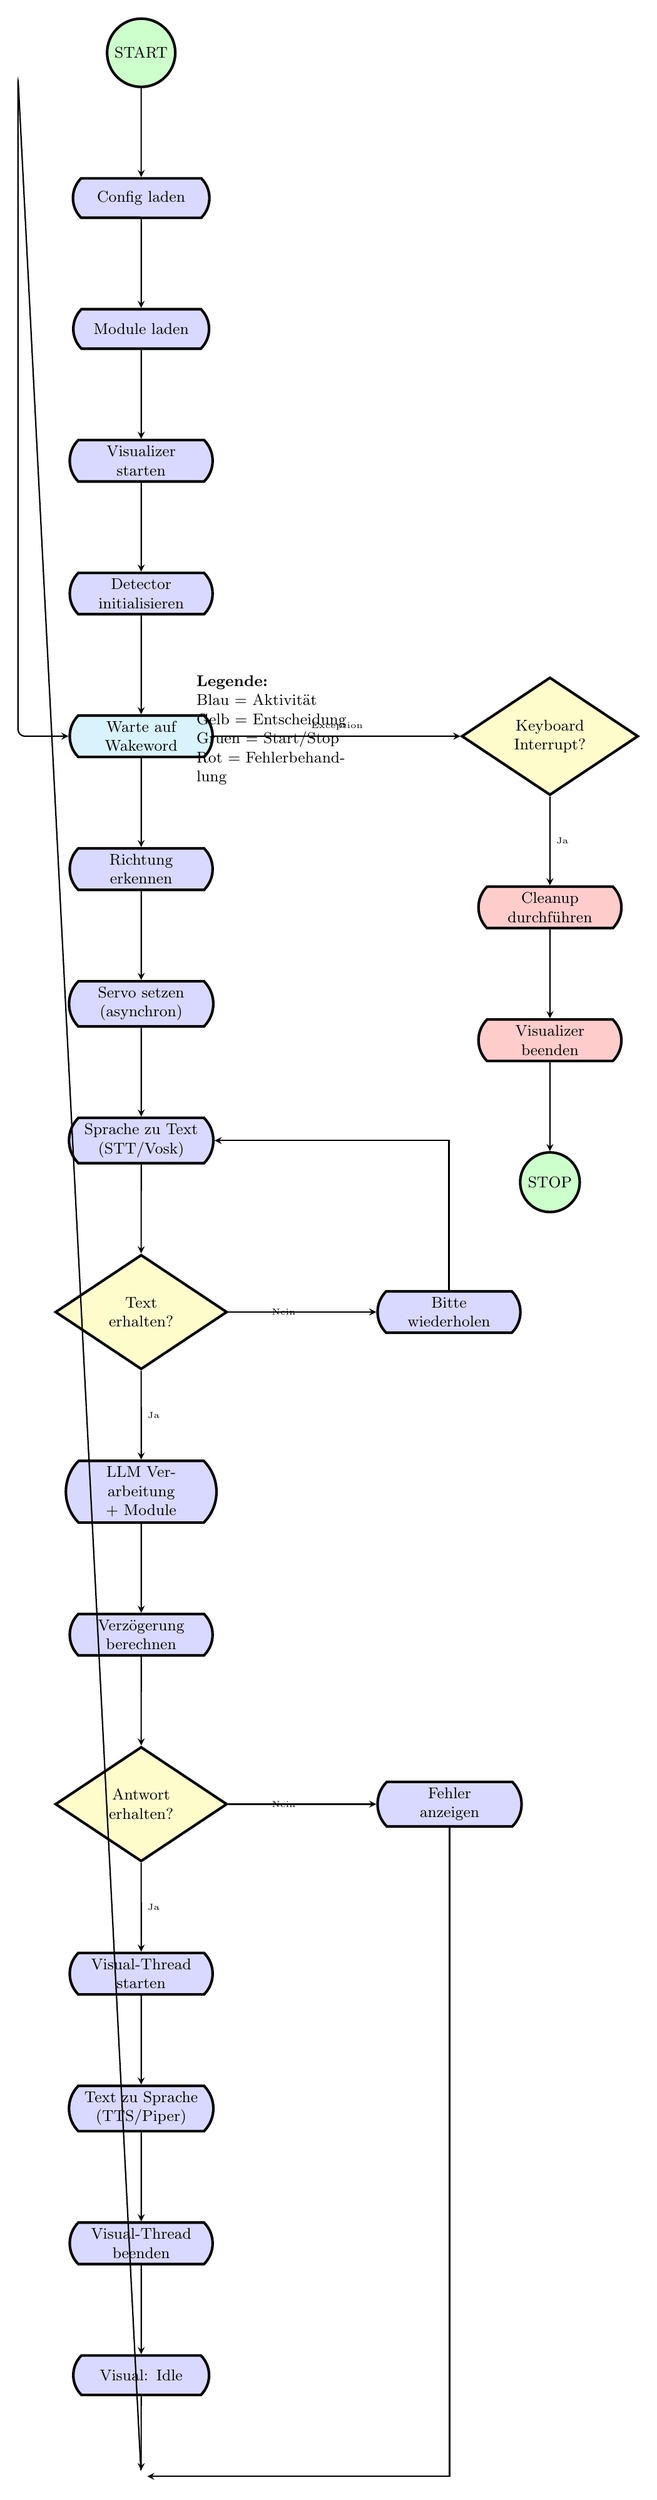
\begin{tikzpicture}[node distance=1.8cm]

% Start
\node[start_end] (start) {START};

% Initialisierung
\node[activity, below=of start] (config) {Config laden};
\node[activity, below=of config] (modules) {Module laden};
\node[activity, below=of modules] (visualizer) {Visualizer\\starten};
\node[activity, below=of visualizer] (detector) {Detector\\initialisieren};

% Hauptschleife
\node[activity, below=2cm of detector, fill=cyan!15] (wait_wakeword) {Warte auf\\Wakeword};
\node[activity, below=of wait_wakeword] (detect_angle) {Richtung\\erkennen};
\node[activity, below=of detect_angle] (servo_set) {Servo setzen\\(asynchron)};

\node[activity, below=of servo_set] (stt) {Sprache zu Text\\(STT/Vosk)};

\node[decision, below=of stt] (check_input) {Text\\erhalten?};
\node[activity, right=3cm of check_input] (retry_stt) {Bitte\\wiederholen};

\node[activity, below=of check_input] (llm) {LLM Verarbeitung\\+ Module};
\node[activity, below=of llm] (calc_delay) {Verzögerung\\berechnen};

\node[decision, below=of calc_delay] (check_response) {Antwort\\erhalten?};
\node[activity, right=3cm of check_response] (error_handle) {Fehler\\anzeigen};

\node[activity, below=of check_response] (visual_thread) {Visual-Thread\\starten};
\node[activity, below=of visual_thread] (tts) {Text zu Sprache\\(TTS/Piper)};
\node[activity, below=of tts] (cancel_thread) {Visual-Thread\\beenden};
\node[activity, below=of cancel_thread] (visual_reset) {Visual: Idle};

% Schleife zurück
\node[below=1.5cm of visual_reset] (loop_back) {};

% Exception Handling
\node[decision, right=5cm of wait_wakeword] (check_interrupt) {Keyboard\\Interrupt?};
\node[error, below=of check_interrupt] (cleanup) {Cleanup\\durchführen};
\node[error, below=of cleanup] (shutdown) {Visualizer\\beenden};

% End
\node[start_end, below=of shutdown] (end) {STOP};

% VERBINDUNGEN - Initialisierung
\draw[flow] (start) -- (config);
\draw[flow] (config) -- (modules);
\draw[flow] (modules) -- (visualizer);
\draw[flow] (visualizer) -- (detector);
\draw[flow] (detector) -- (wait_wakeword);

% VERBINDUNGEN - Hauptschleife
\draw[flow] (wait_wakeword) -- (detect_angle);
\draw[flow] (detect_angle) -- (servo_set);
\draw[flow] (servo_set) -- (stt);

% STT Entscheidung
\draw[flow] (stt) -- (check_input);
\draw[flow] (check_input) -- node[near start, right, font=\tiny] {Nein} (retry_stt);
\draw[flow] (retry_stt) |- (stt);
\draw[flow] (check_input) -- node[right, font=\tiny] {Ja} (llm);

% LLM Verarbeitung
\draw[flow] (llm) -- (calc_delay);
\draw[flow] (calc_delay) -- (check_response);

% Antwort Entscheidung
\draw[flow] (check_response) -- node[near start, right, font=\tiny] {Nein} (error_handle);
\draw[flow] (error_handle) |- (loop_back);
\draw[flow] (check_response) -- node[right, font=\tiny] {Ja} (visual_thread);

% TTS Verarbeitung
\draw[flow] (visual_thread) -- (tts);
\draw[flow] (tts) -- (cancel_thread);
\draw[flow] (cancel_thread) -- (visual_reset);
\draw[flow] (visual_reset) -- (loop_back);

% Schleife zurück zur Hauptschleife
\draw[flow, rounded corners] (loop_back) -- (-2.5,-0.5) |- (wait_wakeword);

% Exception Handling
\draw[flow] (wait_wakeword) -- node[above, font=\tiny] {Exception} (check_interrupt);
\draw[flow] (check_interrupt) -- node[right, font=\tiny] {Ja} (cleanup);
\draw[flow] (cleanup) -- (shutdown);
\draw[flow] (shutdown) -- (end);

% Legende
\node[anchor=north west, text width=3.5cm, font=\small] at (1,-12.5) {
  \textbf{Legende:}\\
  Blau = Aktivität\\
  Gelb = Entscheidung\\
  Gruen = Start/Stop\\
  Rot = Fehlerbehandlung
};

\end{tikzpicture}

\end{document}
